\documentclass[]{beamer}
% Class options include: notes, notesonly, handout, trans,
%                        hidesubsections, shadesubsections,
%                        inrow, blue, red, grey, brown

% Theme for beamer presentation.
\usepackage{beamerthemesplit}
\usepackage{comment} 
\usepackage{blindtext}
% Other themes include: beamerthemebars, beamerthemelined, 
%                       beamerthemetree, beamerthemetreebars  

\title{Type the TITLE of your project here}    % Enter your title between curly braces
%\author{Presented by :-}
\author{Under the Supervision of \\ Guide's Name, Asst. Prof., CSE Dept. \\ Presented by :- \\ ABC(11UCS001) \\ DEF(11UCS002)\\ GHI(11UCS003) \\ JKL(11UCS004) \\ MNO(11UCS005) \\ PQR(11UCS006)}
%\institute{\normalsize NIT Agartala}
%\date{Nov 20, 2014}                    % Enter the date or \today between curly braces

\begin{document}

% Creates title page of slide show using above information
\begin{frame}
  \titlepage
\end{frame}
\note{Talk for 30 minutes} % Add notes to yourself that will be displayed when
                           % typeset with the notes or notesonly class options

\section[Outline]{}

% Creates table of contents slide incorporating
% all \section and \subsection commands
\begin{frame}
  \tableofcontents
\end{frame}


%\section{Simple slide with three points shown all at once}
\section{Introduction}
\begin{frame}
  \frametitle{Introduction}   % Insert frame title between curly braces

\begin{itemize}
\item  .....................
\item  ............................
\item  ..................
\end{itemize}
\end{frame}
\note[enumerate]       % Add notes to yourself that will be displayed when
{                      % typeset with the notes or notesonly class options
\item Note for Point 1   
\item Note for Point 2   
}


\section{Type the name of next topic}
\begin{frame}
\frametitle{Type the name of next topic}
\begin{itemize}
\item ..............
\item ...............
\item ................. 
\end{itemize}
\end{frame}

\section{Type the name of next topic}
\begin{frame}
\frametitle{Type the name of next topic}
................................................................
...............................................................
\begin{itemize}
\item<1-> abc: .................... 
\item<2->xyz: ......................
\item<3->pqr: ........................ 
\end{itemize}
\end{frame}
\begin{frame}
\frametitle{contd.}
.................................
\begin{itemize}
\item<1-> def 
\item<2-> ghi
\item<3-> jkl
\end{itemize}
\end{frame}

\begin{frame}
\frametitle{Type the name of next topic}
\begin{itemize}
\item ........................
\item ........................
\end{itemize}
\end{frame}

\begin{frame}
\frametitle{Type the name of next topic}
If (abc) \{
\begin{itemize}
\item<1-> ..................... 
\item<2-> .......................
\item<3-> ........................
\end{itemize}
\end{frame}

\begin{frame}
\frametitle{contd.}
\begin{itemize}
\item<1-> .......................
\item<2-> ...................
\end{itemize}
\end{frame}

\begin{frame}
\frametitle{Type the next topic}
\begin{itemize}
\item<1-> .......................
\begin{equation}
W_{i} = C1 * (RE_{i} /MaxRE) + C2 * (HC_{i} /MaxHC)
\end{equation}  
Where $|C1|+|C2|=1 .$


\end{itemize}
\end{frame}

\begin{frame}
\frametitle{Contd.}
.......................................
\end{frame}


\begin{frame}
\frametitle{Type the next topic}
\begin{itemize}
\item .............................. 
\item ............................
\end{itemize}
\end{frame}
 



\section{Type next section name}
\begin{frame}
\frametitle{Type name of frame}
\begin{tabular}{|c|c|}
\hline
....... & ............\\
\hline
............ & ........\\
\hline
............. & .........\\
\hline
.............. & ...........\\
\hline
.......... & .................\\
\hline
.......... & ................\\
\hline
................ & .............\\
\hline
............. & ..............\\
\hline
.............. & ..................\\
\hline
............... & .................\\
\hline
\end{tabular}
\end{frame}

\begin{frame}
\frametitle{Contd.}
\begin{tabular}{|c|c|}
\hline
.............. & ............\\
\hline
........... & ..............\\
\hline
............ & ..............\\
\hline 
........... & ................\\
\hline
........... & ...........\\
\hline
............ & ............\\
\hline
.............. & ..............\\
\hline
.............. & ...............\\
\hline
............ & ..........\\
\hline
............. & ..........\\
\hline
\end{tabular}
\end{frame}

\section{Results and Discussion}

\begin{frame}
\frametitle{Type name of frame}
\begin{itemize}
\item Throughput - .....................
\item Packet Delivery Ratio (PDR)- ..................
\item Routing Overhead, RO - ...................
\end{itemize}
\end{frame}




\begin{frame}
\frametitle{Type name of frame}
.......................
\begin{figure}
\begin{center}
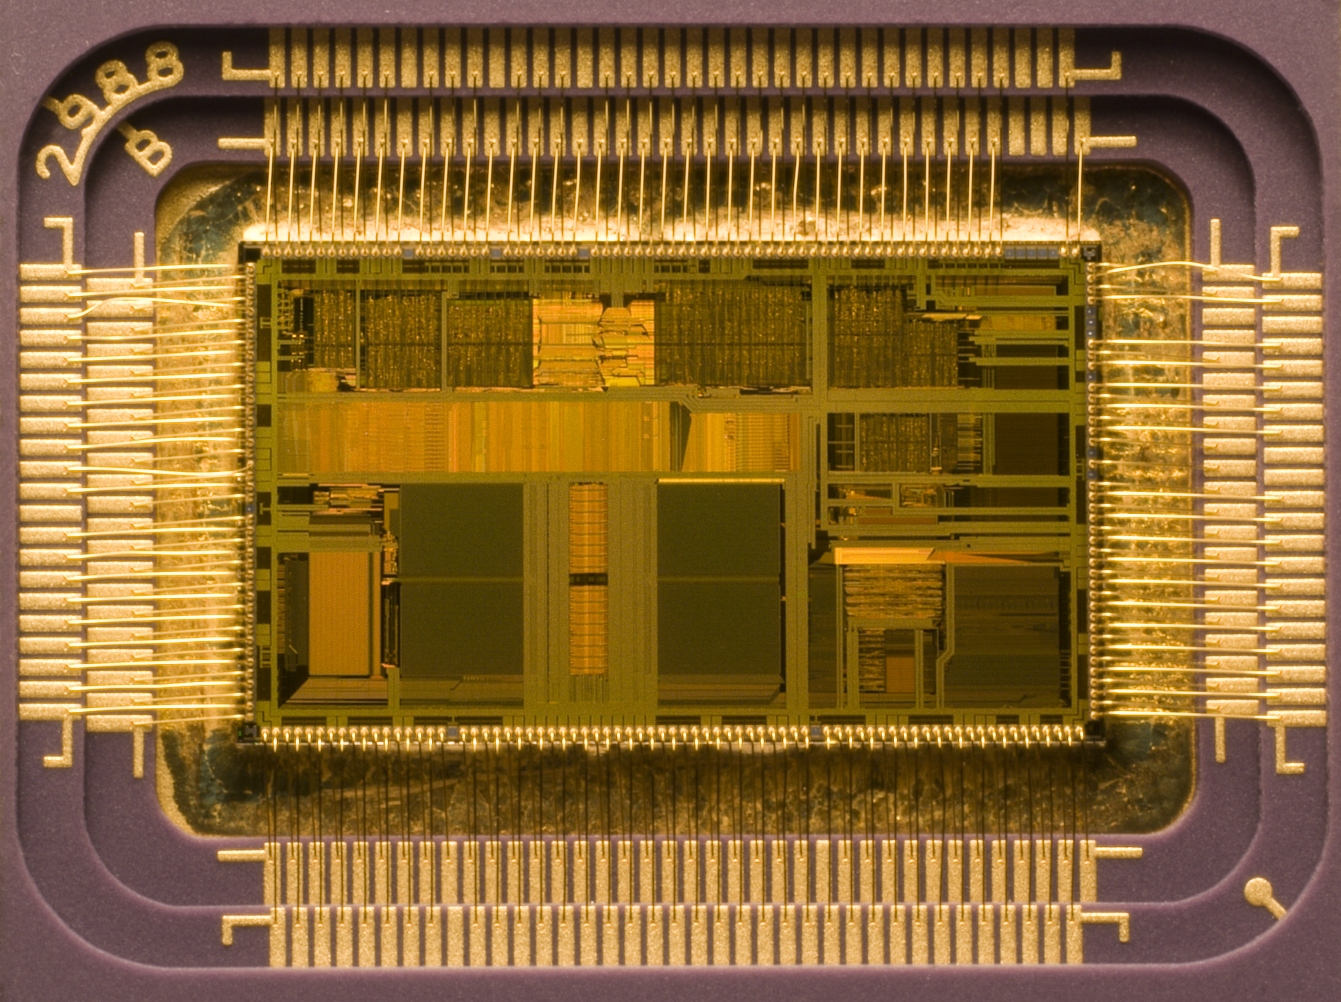
\includegraphics[scale=.5]{def}
\caption{Type the Caption of the figure}
\end{center}
\end{figure}
\end{frame}





\begin{frame}
\frametitle{Type name of frame}
\begin{figure}
\begin{center}
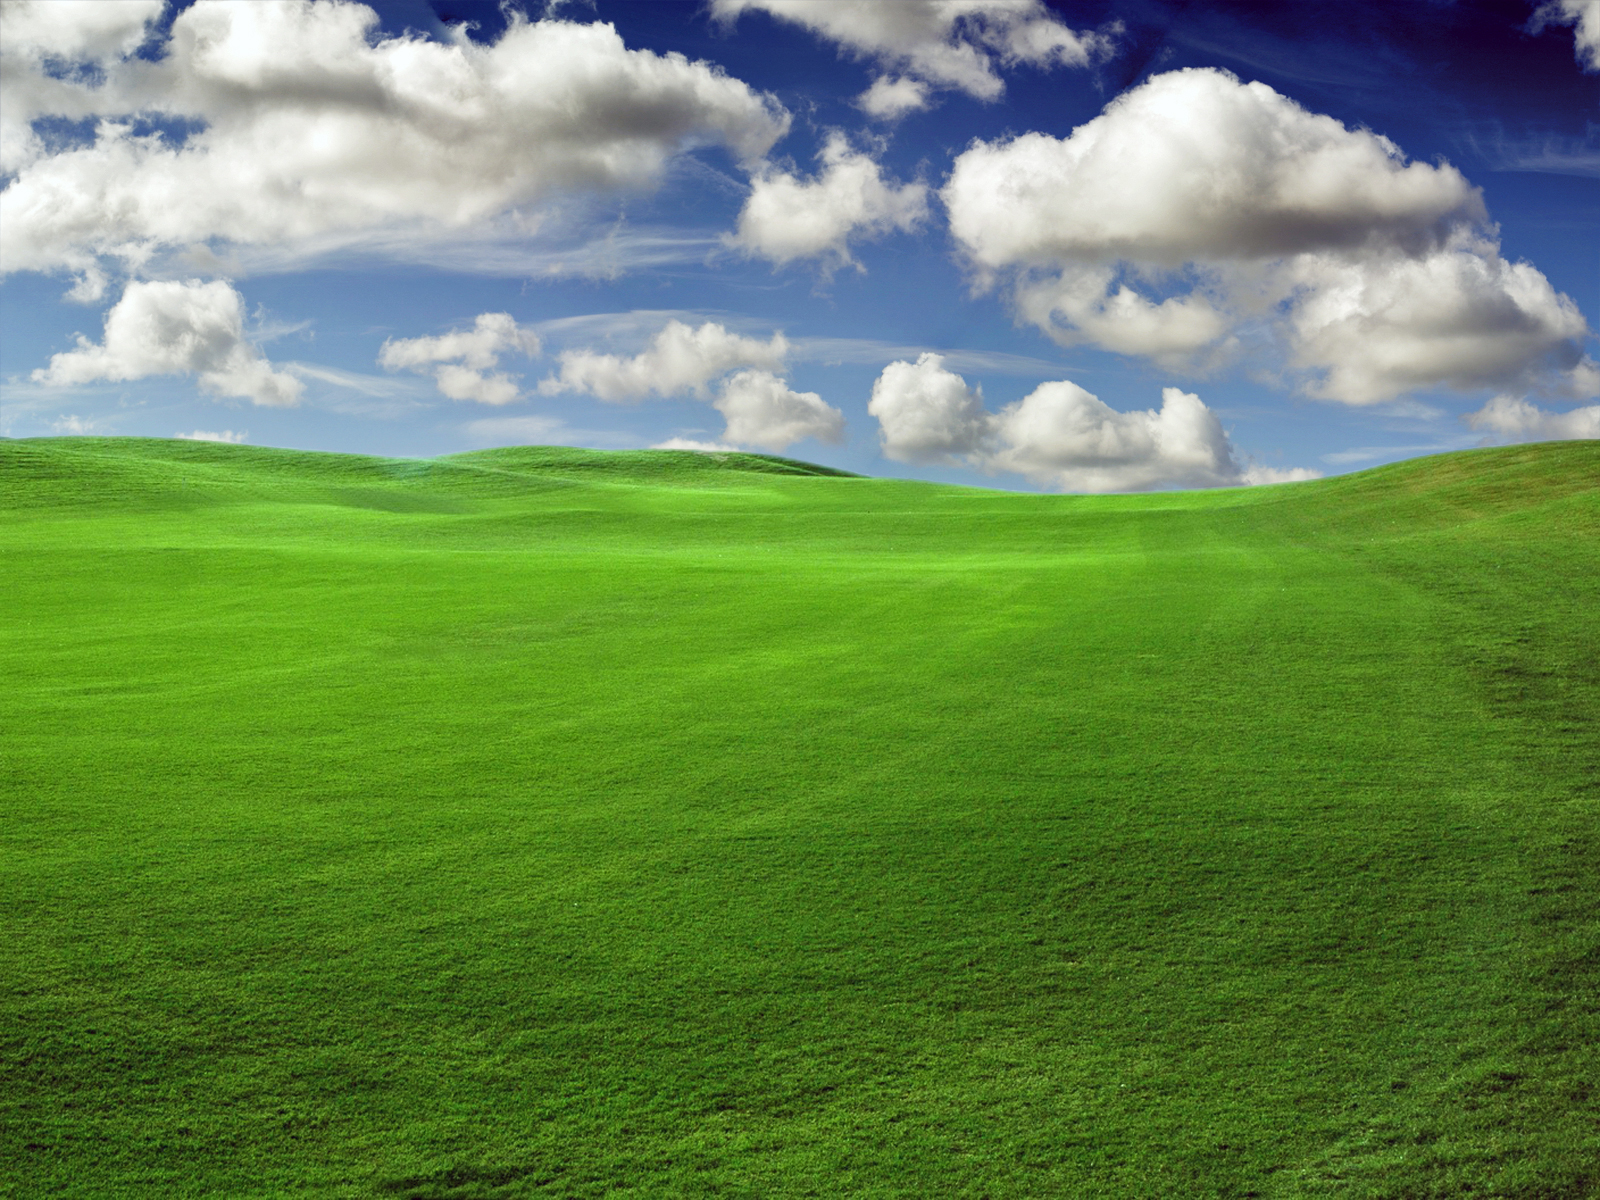
\includegraphics[scale=.1]{mno}
\caption{Type the caption of figure}
\end{center}
\end{figure}
\end{frame}

\begin{frame}
\frametitle{Type name of frame}
\begin{figure}
\begin{center}
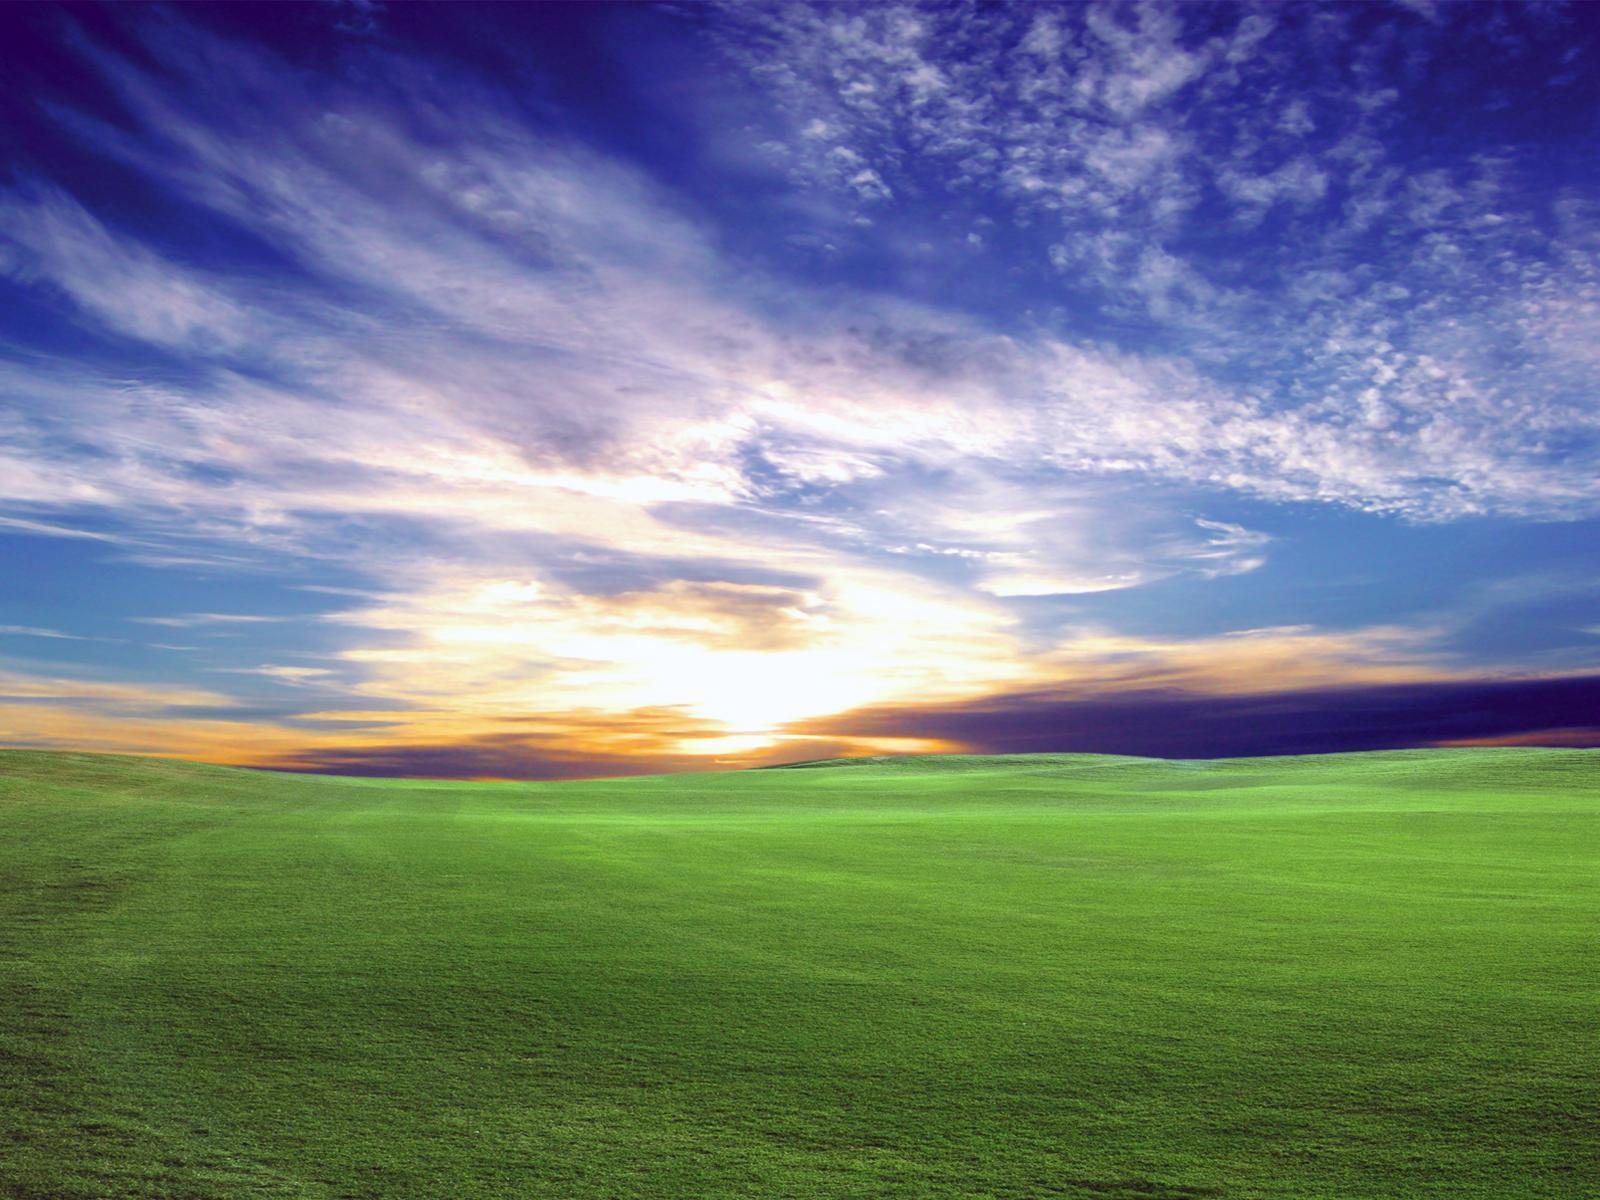
\includegraphics[scale=.1]{pqr}
\caption{Type the caption of figure}
\end{center}
\end{figure}
\end{frame}

\begin{frame}
\frametitle{Type name of frame}
\begin{figure}
\begin{center}

\includegraphics[scale=.1]{stu}
\caption{Type the caption of figure}
\end{center}
\end{figure}
\end{frame}

\section{Conclusion \& Future Work}
\begin{frame}
\frametitle{Conclusion}
\begin{itemize}
\item ......................
\item .....................
\item ........................
\end{itemize}
\end{frame}

\begin{frame}
\frametitle{Future Work}
\Blindtext
\end{frame}

\section{References}
\begin{frame}
\frametitle{References}
\begin{itemize}

\item G. Chakrabarti, and S. Kulkarni, \lq\lq Load Balancing and Resource Reservation in Mobile Ad hoc networks \rq\rq, Elsevier Ad Hoc Networks, accepted 14 April, 2004.

%\item Charles E. Perkins, \lq\lq Ad Hoc Networking", Addison Wesley, USA, 2001.
\item S. Takahashi, J. Hakoda, H. Uehara, and M. Yokoyama, \lq\lq A Load Balanced Routing Scheme for Mobile Ad Hoc Networks", ISITA2004, Parma, Italy, Oct. 2004.

%\item David B. Johnson, Davis A. Maltz, \lq\lq The Dynamic Source Routing Protocol for Mobile Ad hoc Networks", Internet Draft, draft-ietf-manet-dsr-03.txt, Oct. 1999.
\item V. Saigal, A. K. Nayak, S. K. Pradhan, and R. Mall, \lq\lq Load Balanced Routing in Mobile Ad hoc Networks", Elsevier Computer Communications, pp. 295-305, 27(2004).

\item H. Hassanein, and A. Zhou, \lq\lq Load-aware Destination- controlled Routing for MANETs" , Elsevier Computer Communications, pp. 1551-1559, 26(2003).
\end{itemize}
\end{frame}

\begin{frame}
\begin{itemize}
\item N. Wang, Y. Huang and J. Chen, \lq\lq A stable weight-based on- demand routing protocol for mobile ad hoc networks" Information Sciences 177(2007), pp. 5522-5537, 2007.

\item S. Ahn, Y. Lim and J. Choe, \lq\lq A Load-Balancing Approach in Ad-Hoc Networks", ICOIN 2003, LNCS 2662, pp. 672-681, 2003.

\item J-H. Song, V. Wong, and V. C. M. Leung, \lq\lq Load-Aware On- Demand Routing (LAOR) Protocol for Mobile Ad hoc Networks", The 57th IEEE Semiannual Vehicular Technology Conference, pp. 3:1753-1757, 2003.

\item Joo-Han Song, V. W. S. Wong and V. C. M. Leung, \lq\lq Efficient On-Demand Routing for Mobile Ad-Hoc Wireless Access Networks",IEEE GLOBECOM, pp. 558-563, 2003.
\end{itemize}
\end{frame}

\begin{comment}
\begin{frame}
\begin{itemize}
%\item J. Hakoda, H. Uehara, and M. Yokoyama, \lq\lq Performance Evaluation of Mobile Ad Hoc Routing Protocols Based on Link Expiration Time and Load of Node", IEICE Trans. Commun., vol. J85B, no.12, pp. 2108–2118, Dec. 2002.

%\item Y. J. Lee and G. F. Riley, \lq\lq A Workload-Based Adaptive Load- Balancing Technique for Mobile Ad Hoc Networks", IEEE Communication Society, WCNC, pp. 2002-2007, 2005.

\item S. Takahashi, J. Hakoda, H. Uehara, and M. Yokoyama, \lq\lq A Load Balanced Routing Scheme for Mobile Ad Hoc Networks", ISITA2004, Parma, Italy, Oct. 2004.

%\item K. Wu, J. Harms, \lq\lq Load Sensitive Routing for Mobile Ad Hoc Networks", Proc. IEEE ICCCN'01, Phoenix, AZ, pp. 540- 546, Oct. 2001.
\end{itemize}
\end{frame}

\begin{frame}
\begin{itemize}
%\item P. P. Pham and S. Perreau, \lq\lq Increasing the network performance using multi-path routing mechanism with load balance", Ad Hoc Networks, vol. 2, issue 4, pp. 433-459, Oct. 2004.

\item Jin-Woo Jung, Dae In Choi, Keumyoun Kwon, Ilyoung Chong, Kyungshik Lim, Hyun-Kook Kahng, \lq\lq A Correlated Load Aware Routing Protocol in Mobile Ad Hoc Networks",
ECUMN 2004, LNCS 3262, pp. 227–236, 2004.

%\item S. J. Lee, M. Gerla, \lq\lq Dynamic Load Aware Routing in Ad Hoc Networks", Proc. ICC 2001, Helinski, Finland, pp. 3206-3210, June 2001.

\item V. Saigal, A. K. Nayak, S. K. Pradhan, and R. Mall, \lq\lq Load Balanced Routing in Mobile Ad hoc Networks", Elsevier Computer Communications, pp. 295-305, 27(2004).
%\item H.K. Cho, E. S. Kim, and D-W Kang, \lq\lq A Load-balancing Routing Considering Power Conservation in Wireless Ad-Hoc Networks", Proc. Of the 16th International Workshop on Database and Expert Systems Applications, DEXA’05.
\end{itemize}
\end{frame}


\begin{frame}
\begin{itemize}
\item V. Saigal, A. K. Nayak, S. K. Pradhan, and R. Mall, \lq\lq Load Balanced Routing in Mobile Ad hoc Networks", Elsevier Computer Communications, pp. 295-305, 27(2004).
\end{itemize}
\end{frame}
\end{comment}



\begin{frame}
\begin{center}
\huge THANK YOU !
\end{center}
\end{frame}

\end{document}
